\section{Background}
\label{chap:background}
This section will explain swarming and swarm robots. How to implement bird flocking behavior on particles in simulation, and the Boids behavior. It will explain how fish schooling and ant swarm works as well to compliment the bird flocking.

\subsection{Swarming}
Swarm, swarming, swarm intelligence, swarm optimization or swarm robotics are terms used for simple (preferably cheap) robots which can only do simple tasks. However the power of these robots lies in the numbers. The robots might not be able to do an advanced task alone, but together they might be able complete advanced tasks. For instance, one robot might not be able to push a heavy box by itself, but with the help of other robots they might be able to push the box.
Each robot are allowed to communicate with each other, but they do not need to communicate. There are no centralized controller that controls the robot, each one needs to find out what it needs to do by itself or by communicating with the other robots. The idea behind these simple cheap robots are that they can easily be mass produced, interchangeable, modularized and disposable. If one robot is malfunctioning or broken, it would not affect the rest of the swarm. It is therefore no single point of failure in a swarm, and the system is very scalable because robots can easily be added to the system.
Swarm robotics are often very computer efficient, because they each have their own processor. This reduces the computational overhead. 

\subsection{Boids}
In 1986, Craig W. Reynolds created something he called Boids, which stands for \textbf{B}ird-\textbf{oid} object\textbf{s}. Boids are particles that would behave like birds, they would try to flock and fly together without colliding. This was done by using 3 simple behaviors;
\begin{description}
    \item[Separation]
        Each individual will steer away from the other individual if they were too close to each other. This ensure that they do not collide with their neighbors.
    \item[Alignment]
        In a neighborhood (for instance a radius around the individual or the $X$ nearest individuals) find the average angle of the neighborhood and align itself so its angle matches the average angle of the neighborhood.
    \item[Cohesion]
        Steer towards the average position of the other individuals in your neighborhood. This makes the Boids stay in the flock.
\end{description}
\begin{figure}[H]
    \centering
    \subfloat[Separation ]{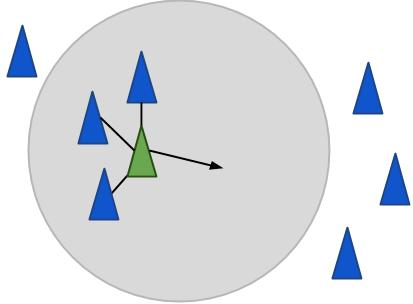
\includegraphics[width=0.3\textwidth]{images/boid_separation.jpg}}
    \hfill
    \subfloat[Alignment ]{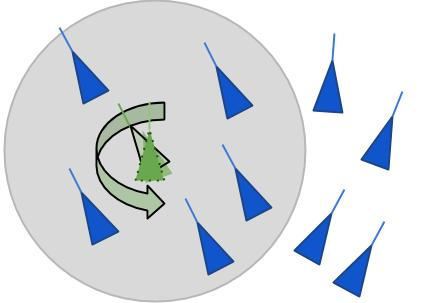
\includegraphics[width=0.3\textwidth]{images/boid_alignment1.jpg}}
    \hfill
    \subfloat[Cohesion ]{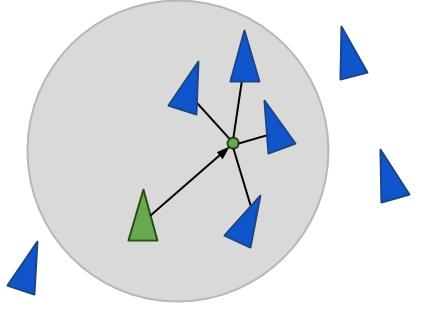
\includegraphics[width=0.3\textwidth]{images/boid_cohesion.jpg}}
            \caption[Boids behavior]{The three behaviors of the Boids}
            \label{fig:boidbehavior}
\end{figure}

The three behavior is per individual Boid, which means that each particle/Boid has to calculate where they are going to fly by checking all the other Boids position and rotation and then act accordingly. Which makes this algorithm $ O(n^2)$ for every frame. 
Reynolds have tried to make the algorithm less computational intensive by putting the Boids into grids with Spatial Hashing. An example of this could be to put all the Boids that has a position $0<x<1$ and $0<y<1$ on the lower left grid, and the ones that has a $1<x<2$ in the next position etc. Using this grid, each Boids in a cell only needs to take the adjacent grids into consideration when checking their neighborhood. That way they do not need to check the position and rotation of all the other Boids.
\begin{figure}[h!]
    \centering
    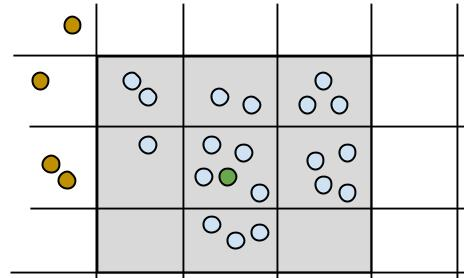
\includegraphics[width=0.8\linewidth]{images/boid_spatialhash}
    \caption{Boids in grids using spatial hash} \label{fig:spatialhash}
\end{figure}
As illustrated in the figure, the green Boid only needs to check the gray Boids that surrounds its own cell, it does not need to check the rotation and position of the orange/brown Boids outside of the gray box, because they are too far away to be considered a part of its neighborhood.

In another paper a different technique were used to optimize 3D swarms, a method using neighborhood grids.\\

Other optimization has been made as well, like the neighborhood grid.
Each Boids to cell ratio would be 1 to 1, that is for every cell, there would be at max 1 Boid. Each Boid would have their respective cell based on their position in space, for instance a Boid with low $x$-value would be on the left of a Boid with higher $x$-value, and Boids who are closer to each other in geometric space would be stored closer to each other in the grid. To obtain this, the Boids needed to be sorted. Odd Even sort and Bitonic sort were used as the sorting algorithm. See appendix \ref{app:sorting}.

Of the two sorting algorithm, Odd Even sort was faster, but not very precise. More than 10\% of the entities were placed in the wrong cell. The paper did an odd even sort algorithm for each axis, that is one odd even sort for x, y and z in parallel.
Bitonic Sort on the other hand was slower, but a lot more precise. Less than 1\% of the entities were placed in wrong cell. The reason for placing a Boid in the wrong cell is due to way the sorting works, it sorts all the entities in one axis first, then a second axis and then the third last axis. For instance sorting on $x$-values first, for the $y$-values, then the $z$-values. When swapping one of the latter axises it might mess up the sorting of one of the other axises.

After the Boids were placed in their corresponding grid, the work could be distributed to the GPU which would calculate where each Boids' new location and rotation would be based on their adjacent neighbor depending on the Moore radius.
The paper tried to vary the number of Boids from 1,000 to 1,000,000 and they had 4 types of Boids. The same types of Boids would try to flock with each other while different types of Boids would try to avoid each other.
They were able to see a speedup compared to the spatial hashing method used by Reynolds, but the Boids were not rendered as a bird or an object, only as a primitive shape. They didn't mention if they tried to add non moving obstacles in their test. Due to the high percentage of Boids being placed in the wrong cell when using odd even sort, a lot of Boids would crash into their neighbor during the test run. However using the neighborhood grid method on GPU, real time simulation of 1 million Boids were possible (6-8 fps).\\

In the paper "steering behaviors for autonomous character" Reynold discusses that an autonomous character, which is a type of autonomous agent are agents that have some ability to improvise their actions. That means that these agents do not have their actions scripted in advance.
It is possible for the Boids to have more behaviors, called steering behaviors \cite{Reynolds1999}. The steering behavior decides where the Boids are supposed to steer after their three simple behavior are satisfied.  These steering behavior can be seek, flee, pursuit, evade etc. 

The \textbf{seek} behavior tells the Boid to seek a goal, it will try to reach the goal/object as fast as possible, and due to the high speed it has when arriving it will fly past the goal. It then turns around to seek the goal again.
A seek behavior should have an \textbf{arrival} behavior to counteract the fly-by, that means that when nearing the goal, the Boid will slow down so it stops at the goal in the end, instead of flying past it.

A \textbf{flee behavior} is almost the same as the seek, except in the opposite direction. It will try to turn away from the "goal" and fly in the opposite direction or rather fly as far away from the "goal" as possible.

\textbf{Pursuit} is the same as seek, except it applies to moving objects. Pursuit requires prediction of the target's future position. The approach is to predict the future position of the target, reevaluate and readjust it each step. A prediction might be wrong at one time step, but this only applies for that single time step, and a new prediction will be made at the next time step which hopefully will be correct.

An \textbf{offset pursuit} behavior behaves almost the same way as the normal pursuit behavior, except that it will not "crash" into the target but have an offset or $R$. An example of this could be an aircraft flying near the sensors of a base or something similar. 




\subsection{Not bumping into things}

In the paper named "not bumping into things" W. Reynolds discusses how to perform obstacle avoidance, that is obstacles that are placed in the environment which is not a Boid. These obstacles are usually static, that is non moving obstacles. He starts out with the idea of a forcefield around the obstacle which he calls the \textit{steer away from surface} approach. The idea is to have every obstacle emit a forcefield around itself which pushed the Boids away. For instance if a Boid is flying toward an obstacle, the obstacle would push the Boid to one side of itself. However this force field method would not work if the Boid flew straight into an obstacle, because the forcefield force would be straight opposite of the direction the Boid is flying thus making the Boid decelerate until it stopped.
The next obstacle avoidance technique Reynold discussed is the curb feeler technique or steer along the wall technique. The idea is to have a feeler that would detect an obstacle before the Boid would crash into it, then turn the Boid away from the obstacle. This can be compared to walking down a dark alleyway where you'll reach your hand out to feel the walls around you and navigates through the alleyway just by feeling the wall(s).
The last technique for navigating and avoiding obstacles discussed in this paper was image processing. Images could processed in real time to a gray scale image where white would signify an obstacle. The algorithm would start with the center of the image, if this was a white pixel it would start to search outwards in a spiral to find either a gray pixel or a black one and then turn the Boid in this direction. This could also be combined with a \textit{Z-buffer image} which gives us a map of the distances to obstacles that lies in front of the Boid, this z-buffer image can be obtained by radar, sonar or similar technology. One interesting way of using the Z-buffer image is to implement a "steer towards the longest clear path". However using this technique without any form of planning or learning might lead the Boid into a local cavity which might be a dead end.

\subsection{Physic based control system}
In the paper Distributed physics-based control of swarms of vehicles by W. Spears and D. Spears a self emergent system is formed using simple attractive and repulsion force for each particle. The idea behind their system was to create an artificial physics framework (AP) that would simulate a physical system. In their paper they had the particles attract other particles that were farther away than distance \textit{r} and a repulsive force is applied if the particles are closer than distance \textit{r}. This leads to the particles always being at distance \textit{r} from each other which will form a hexagonal lattice. In the hexagonal lattice, each particle will be at a distance $r$ away from each other, but the next neighbor will be $\sqrt{3}r$ away, therefore each particle only have a vision range of $1.5r$ so they do not affect the particles that are too far away from it. In the simulation they spawned all the particles in a cluster, using the two-dimensional Gaussian random variable to initialize the position of the particles. The particles starts with a velocity of 0.0, but their framework does not require so. Due to local forces, the particles will disperse and form local hexagons. To evaluate the quality of the lattice they measured the orientation error of the lattice: they took any particles that were $2r$ apart and formed a line segment, then they took any other particles that were $2r$ apart and formed another line segment. The angle between these to line segments should be measured to be a multiple of $60^{\circ}$. The error would be the absolute value of the difference between the measured angle and the nearest multiple of $60^{\circ}$. The error ranges from $0^{\circ}$ to $^{\circ}$, they also checked the size of the particle cluster, for each particle $i$ they counted the number of "close" particles, that is particles that are in the range of $0<r<0.2r$. The minimum cluster size is 1.0 because they count the particle $i$ as well as its neighbors. The cluster count was averaged for all the particles. At the start there were a high cluster count, but it decreased to roughly 2.5 after 6 time steps. 
They also tried out making patterns, but had to introduce a concept of spin; each particle were either spin "down" or spin "up". Opposite spins would attract each other if the distance was greater than \textit{r} and repel each other if the distance is less than \textit{r}. If the particles had opposite spin the distance would be $\sqrt{2}r$. This means that all the vertical particles would be alternating between spin up and spin down, the same goes for the particles in the horizontal space. The diagonal particles on the other hand will have the same spins as their diagonal neighbors. Sometimes the formation would have "holes" in it, so instead of static spins, the particles were allowed to change their spin. This would fill in the holes or flaws in the square lattice, according to their theory.
A particle would only change its spin if it had a very close neighbor ($r<1$), and the probability of changing spin was quite small.


In the paper "V-like formation in flocks of artificial birds" by A. Nathan and V. Barbosa bird flocking is discussed. They ran a simulation that where each bird individual had 3 simple rules: 
\begin{itemize}
    \item Coalescing rule \\
        The birds should try to seek the proximity of the nearest bird.
    \item Gap-seeking rule \\
        If rule 1, the coalescing rule is not applicable anymore the bird should find a position with unobstructed view -  that is, the bird should be able to see in front of it without anything being in the way.
    \item Stationing rule \\
        Try to stay in place.
\end{itemize}
These rules would make sure that the birds were able to flock and form different shapes. The only thing that was common between the different runs in this paper was that the bird behind would be a little bit behind and slightly left or right of the bird in front (following rule \#2). A lot of different shapes was obtained during the runs, the birds flocked and formed a V-shape, a diagonal line, an inverted V-shape etc.

\subsection{Family bird: A heterogenous simulated flock}
This paper says that bird flocks and fish schools seems to be very complex, but the mechanics are very simple as illustrated by Reynold. Only a few simple rules will create flocks that flock together and splits up to avoid obstacles. These flocks are not spectacular or mind blowing compared to the flocks found in nature, due to the rigid motion of each individual. To tackle the artificialness of each individual, Heppner introduced randomness to the motion of the individuals, defending it by saying that these randomness simulates wind gust, random obstacles and other factors. 
However the authors of this paper does not agree with this approach because wind gusts will affect the whole flock, not just a random single individual at random. Even with these randomness added, the flock still does not seem lifelike enough compared to their counterpart found in nature. The reason for the lack of breathtaking in these flocking algorithms are that the individuals all have the same characteristics. In nature each individual will have different size, age, form and shape. 
Usually in flocking algorithms, each individual takes into account where all the other entities are and then act accordingly. In nature, each individual might have limited information about the flock, it might only be able to gain so much from its vision due to other flock members being occluded or not able to hear some of the other individuals due to noise or other factors.
This paper runs a simulation with different types of bird , where social relations are a factor and individuals might be solitary or social. Social individuals are entities who would like to stay close to members of its own social group, for instance a social dove will want to stay with other doves. Solitary individuals on the other hand does not care about staying with its own flock and might drift to another flock. For instance a solitary dove might fly amongst hawks or other types of birds. A flock in this paper are defined as a group where the individuals affect each other in the same group. The simulation they ran varied between all solitary birds to 4 types of different social birds.

\subsection{Particle Swarm Optimization}
Swarms has a lot of potential, not necessary only on robotics but swarms can be used to optimize problem, hence the name particle swarm optimization (PSO). PSOs are used to solve problems where optimization are needed. The idea behind PSOs are to have a swarm of particles spawn at random positions in the search space, and then let them fly around searching for solutions. Each particle will know the best solution it have found so far, and the best solution that is found globally. In some PSO implementations a local best found solution is also known amongst the individual. This local best solution is the best solution amongst a subgroup of individuals and can change for a particle depending on the position of the particle.

\subsection{Other swarming animals}
\subsubsection{fishes}
In this paper Xiaoyuan Tu explains how fishes form schools and how different intentions make the fish behave the way they do. He starts out with explaining how a fish and how the simulator is constructed, the math behind it and how the motor controllers work. For the simulation there's different types of fishes, some of them are predators and some of them are preys. The name explains itself, but to be clear, predators are larger fishes which tries to eat other smaller preys. Each fish has a 300 degrees, where it can see in front of it and has a blind spot directly behind it. 
The range of the vision is also limited and might be occluded by other objects. Each fish has a intention generator, which basically is a flowchart of what the fish needs to do. The prey and predator fish have different intention generators. The predators do not get preyed upon, and thus does not need to look out for other predators, therefore are the intentions of escaping, mating and schooling with other fishes of the same species are disabled. The reason for disabling mating is because there's no need for new predator fishes because they don't die in this simulation. They also don't need to school with other predators because they are not in danger, and don't need the extra survivability.\\
Whenever a predator sees a prey it will chase the prey if the cost of reaching it is minimal, if it's too much, it will not bother chasing. \\
Preys on the hand needs the extra survivability, and will try to school with the other fishes if it detects a predator nearby. Each fish will then try to stay a certain distance from each other, which is roughly on body length in distance. Then the fishes will try to adjust its speed and direction so it matches the other members. When this school of fish encounter an obstacle, they individual fishes will try to avoid this obstacle, this might lead to the school splitting up and rejoining after they have avoided the obstacle. \\
A third type of fish introduced here are the pacifists fish. This one differs from the other two type in that the intention of mating is activated while escaping and schooling are deactivated.
The paper describes that there are male and female fishes, and the two behavior which can occur when the fishes start to mate. A behavior named \textit{nuzzling} where the male fish seeks the female and nudges her abdomen until she's ready to spawn, and \textit{spawning ascent} where the female swims repeatedly to the surface while releases gametes. The paper also describes in detail how the fishes select potential partners and how they try to impress each other for mating purposes.

\subsubsection{Ant swarms/colonies}
Ant swarms behaves differently than other types of swarms, ants do not try to form formations for survival in the same way that birds and fishes do. Ant swarming are mostly about their foraging behavior, that is how they find food for their colony. Each ants' goal is the survival of the colony rather than the survival of each individual. When ants tries to find food, they scatter the area by walking in random manner. While exploring the ants leave behind a chemical on the ground, a so called pheromone that the other ants will be able to feel/smell. This pheromone will slowly but surely dissipate. Whenever the explorer ant find a food source, it will evaluate the quality of the food before returning to the anthill. During the return trip, pheromones are reapplied to the path, but the amount is adjusted based on the evaluation of the food, better food will yield higher pheromone. This method will ensure that the rest of the ants will take the shortest path from the anthill to the food. For the artificial ants, the ant system uses a graph $G = (V,E)$ to model the paths, $V$ is the nodes and $E$ are the edge(s) between the nodes. In the paper "REF ants", they use two nodes, namely $v_s$ which is the starting node or anthill. The node $v_d$ is the food source. There is two ways to reach the food source from the anthill, $e_1$ and $e_2$, which have lengths $l_1$ and $l_2$ where $l_2 > l_1$. A value $\tau_i$ denoted the artificial pheromone, and it indicates the strength of the pheromone. 

An ant will choose a path with the probability $p_i = \frac{\tau_i}{\sum_{ n = 1}^{k}\tau_n}$ where $k$ denotes the number of paths. In the paper REF, they only have two paths, so the probability of choosing a path is $p_i = \frac{\tau_i}{\tau_1 + \tau_2}, i = 1,2$.
The ant will probably choose $e_1$ if $\tau_1 > \tau_2$ and vice versa.
The ants will return using the same path as the one it took, and reinforce the path with new pheromones using the formula $\tau_i \leftarrow \tau_i + \frac{Q}{l_i}$ where $Q$ is a positive constant. The pheromones that have already been laid out in the path will slowly evaporate, the evaporation formula used is $\tau_i \leftarrow (1-\rho)\cdot\tau_i, i = 1,2$, where $\rho \in (0,1]$. These math formulas will over time make sure that the ants are converging to the short path.

The biggest difference between these artificial ants and real ones are that these move synchronously, while real ants are asynchronous. Real ants leaves pheromones on the ground whenever they move, these artificial ones only leave behind the pheromones on the way back to the anthill. The normal ants' pheromone strength are due to evaporation, while the artificial ones regulates the strength of the pheromones using an evaluation of some quality measure. The ant system can be used for approximate algorithms for combinatorial optimization problem, especially for combinatorial problems which are NP-hard.